%\color{cyan} %color de texto con 70-80 % o más de avance
\section{Análisis de Plataformas de Sensado Remoto}
En esta sección se realiza un análisis de factibilidad y conveniencia de las plataformas de adquisición de imágenes aéreas, considerando las características propias de las reservas de bosques nativos de la provincia de Misiones.\\

\subsection{Reservas de bosque nativo de la Selva Paranaense en la Provincia de Misiones}
En primer lugar, se hace una descripción de las características de las reservas de bosque nativo en la provincia de Misiones. Esta parece ser una restricción geográfica importante, pero en la provincia de Misiones está presente casi la mitad del remanente en pie del bioma conocido como Bosque Atlántico o Selva Paranaense, que representa hoy en día solo un 5\% de la extensión histórica, que cubría el nordeste de Argentina, buena parte del Paraguay y el sur de Brasil. 

A partir de información publicada por el Ministerio de Ecología y Recursos Naturales Renovables de la Provincia de Misiones \cite{noauthor_areas_nodate}, la Red Argentina de Reservas Privadas \cite{noauthor_red_nodate} y diversas noticias publicadas en medios digitales, se realizó una base de datos de las reservas de la provincia. Esta información se dejará disponible a través del repositorio de la UNaM \cite{noauthor_principal_nodate}.
Se lista un total de 126 reservas, clasificadas según  su pertenencia, privada o pública, y dentro de esta última, según su jurisdicción: nacional, provincial y municipal. En el Apéndice es presentado un listado completo.
A fines de relevamiento y monitoreo, una de las principales variables que influyen es el tamaño de la reserva, por lo tanto, se toma este parámetro para proponer una clasificación entre reservas de pequeña extensión (menor a 200 ha), mediana extensión (de 200 a 2.000 ha) o gran extensión (mayor a 2.000 ha). En la Figura \ref{hist_res} se muestra un histograma indicando la cantidad de reservas en cada grupo. Resulta evidente que la mayor cantidad de reservas son de pequeña extensión, representando el 56\%.
%%%%%%%%%%%%%%%%%%%%%%%%%%%%%%%%%%%%%%%%%%%%%%%%%%%%%%%%%%%%%%%%%%%%%%%%%%%%%%%%%%%%%%%%%%%%%%%%%%%%%%%%%  
\begin{figure}[h!]
    \centering
    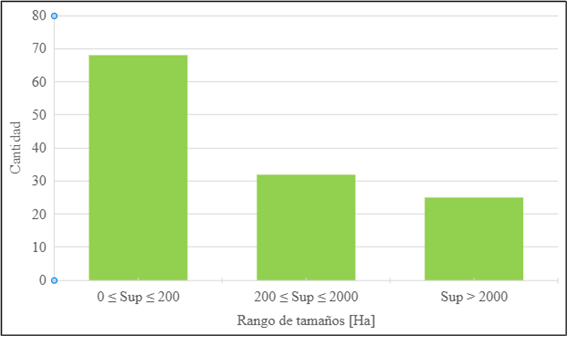
\includegraphics[width=0.5\textwidth]{Imagenes/histograma_reservas.png}
     \hfill
     \caption{Histograma de reservas de la provincia de Misiones}
    \label{hist_res}
\end{figure}
%%%%%%%%%%%%%%%%%%%%%%%%%%%%%%%%%%%%%%%%%%%%%%%%%%%%%%%%%%%%%%%%%%%%%%%%%%%%%%%%%%%%%%%%%%%%%%%%%%%%%%%%



Algunas de las reservas encontradas en la provincia de Misiones son descritas a modo ilustrativo a continuación.

\subsubsection{Reserva Biósfera Yaboty}
La Biosfera Yaboty, está integrada por un conjunto de reservas públicas y privadas cuya extensión es totaliza 253.773 ha [1]. Está enclavada en el centro-este de la provincia.
\begin{table}[H]
    \centering
    \begin{tabular}{|c|c|c|}
        \hline
        \textbf{Reserva} & Biósfera Yaboty &   \multirow{ 3}{*}{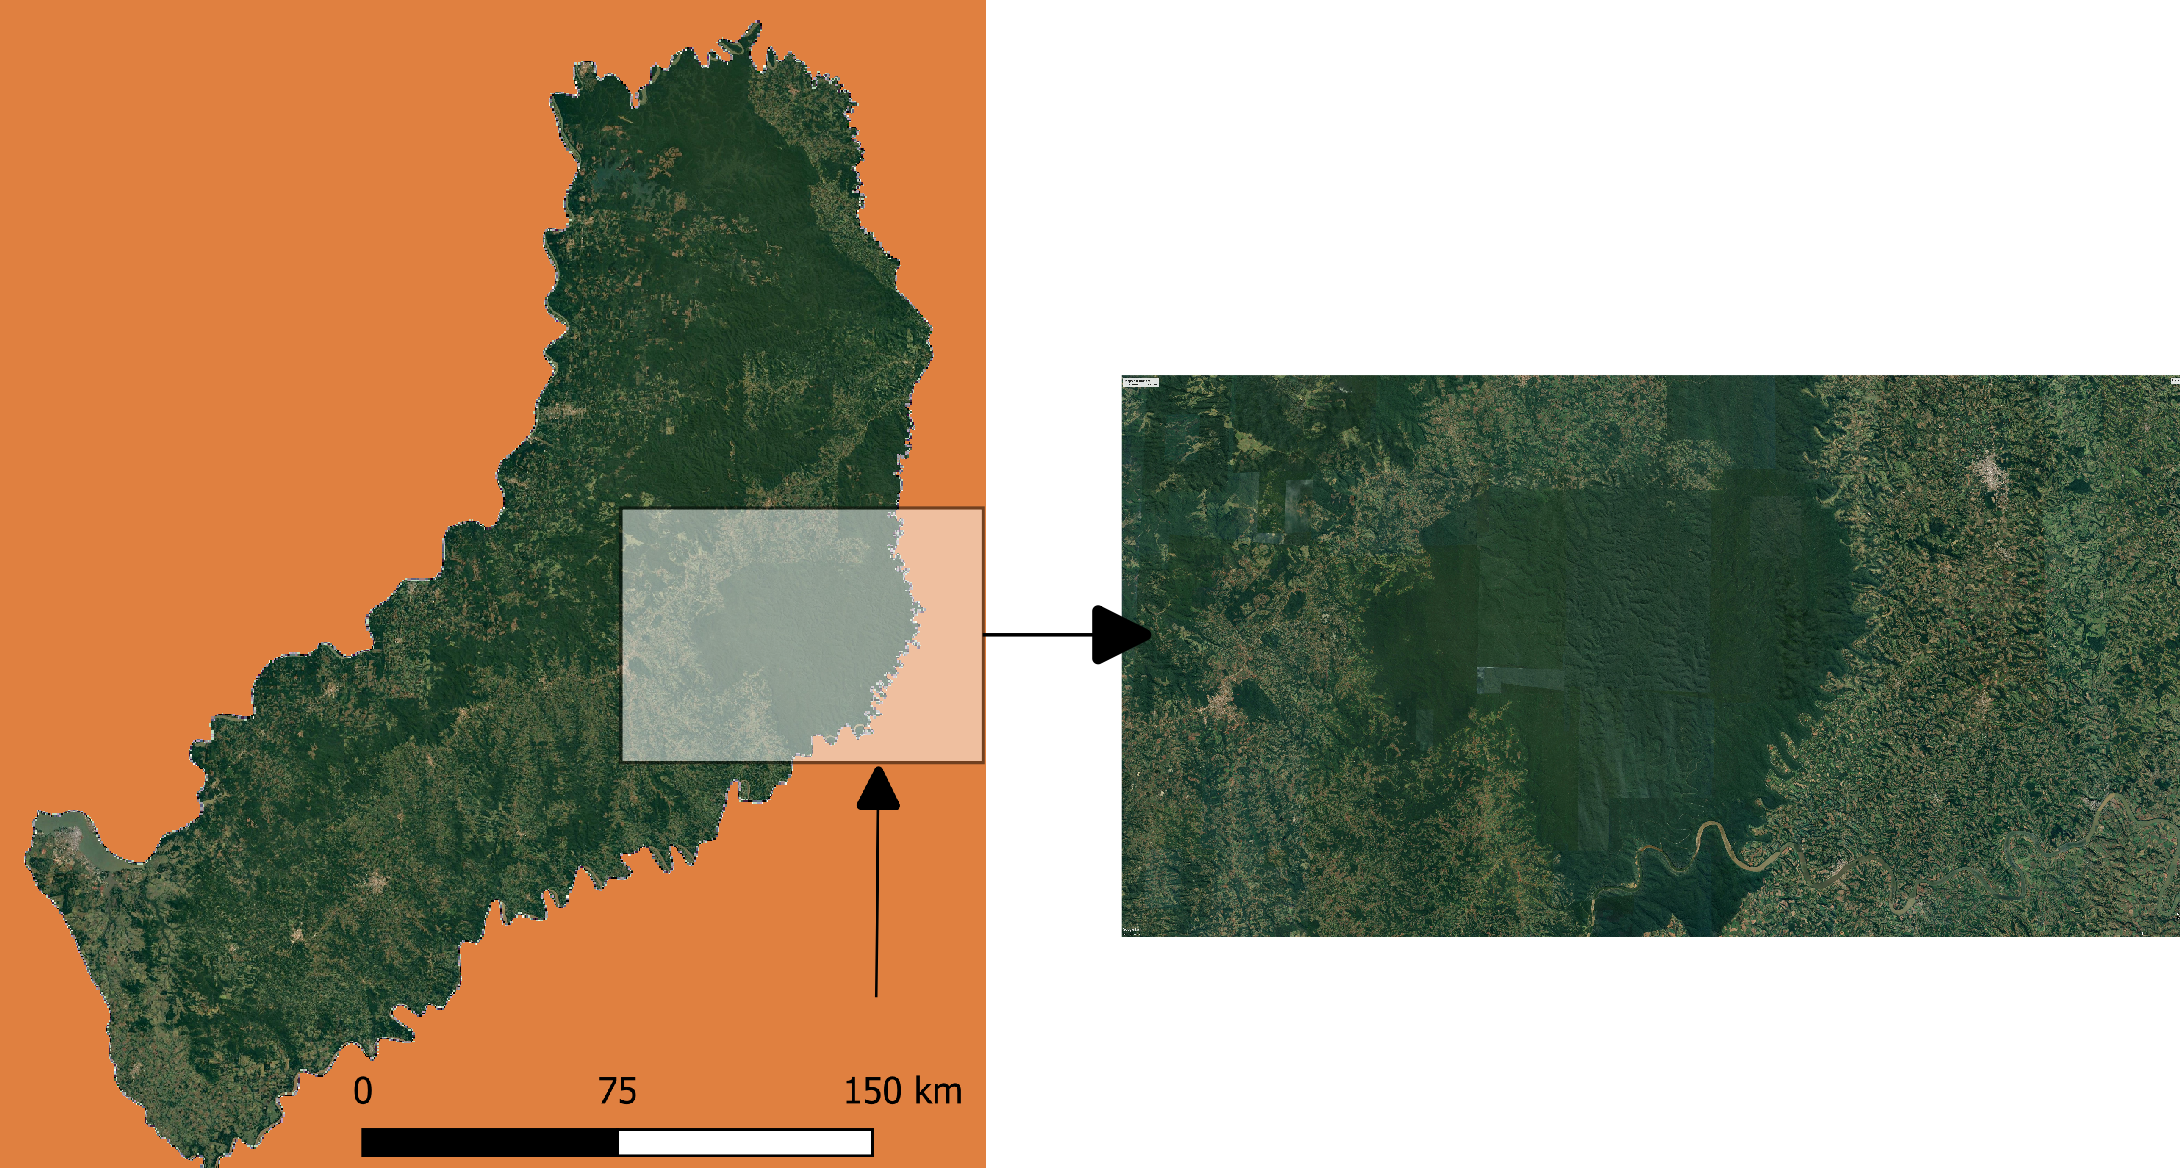
\includegraphics[width=30mm]{Imagenes/Yaboty.png}}\\ 
        \textbf{Administración} & Pública\\
        \textbf{Ubicación} & E 53° 40’, O 54° 18’, N 26° 37’ S 27° 12’ \\
        \textbf{Superficie} & 253.773 ha\\
        \hline
    \end{tabular}
    \label{Yaboty}
\end{table}

\subsubsection{Reserva San Sebastián de la Selva}
\begin{table}[H]
\centering
\begin{tabular}{|c|c|c|}
\hline
 \textbf{Reserva} & San Sebastián de la Selva &   \multirow{ 3}{*}{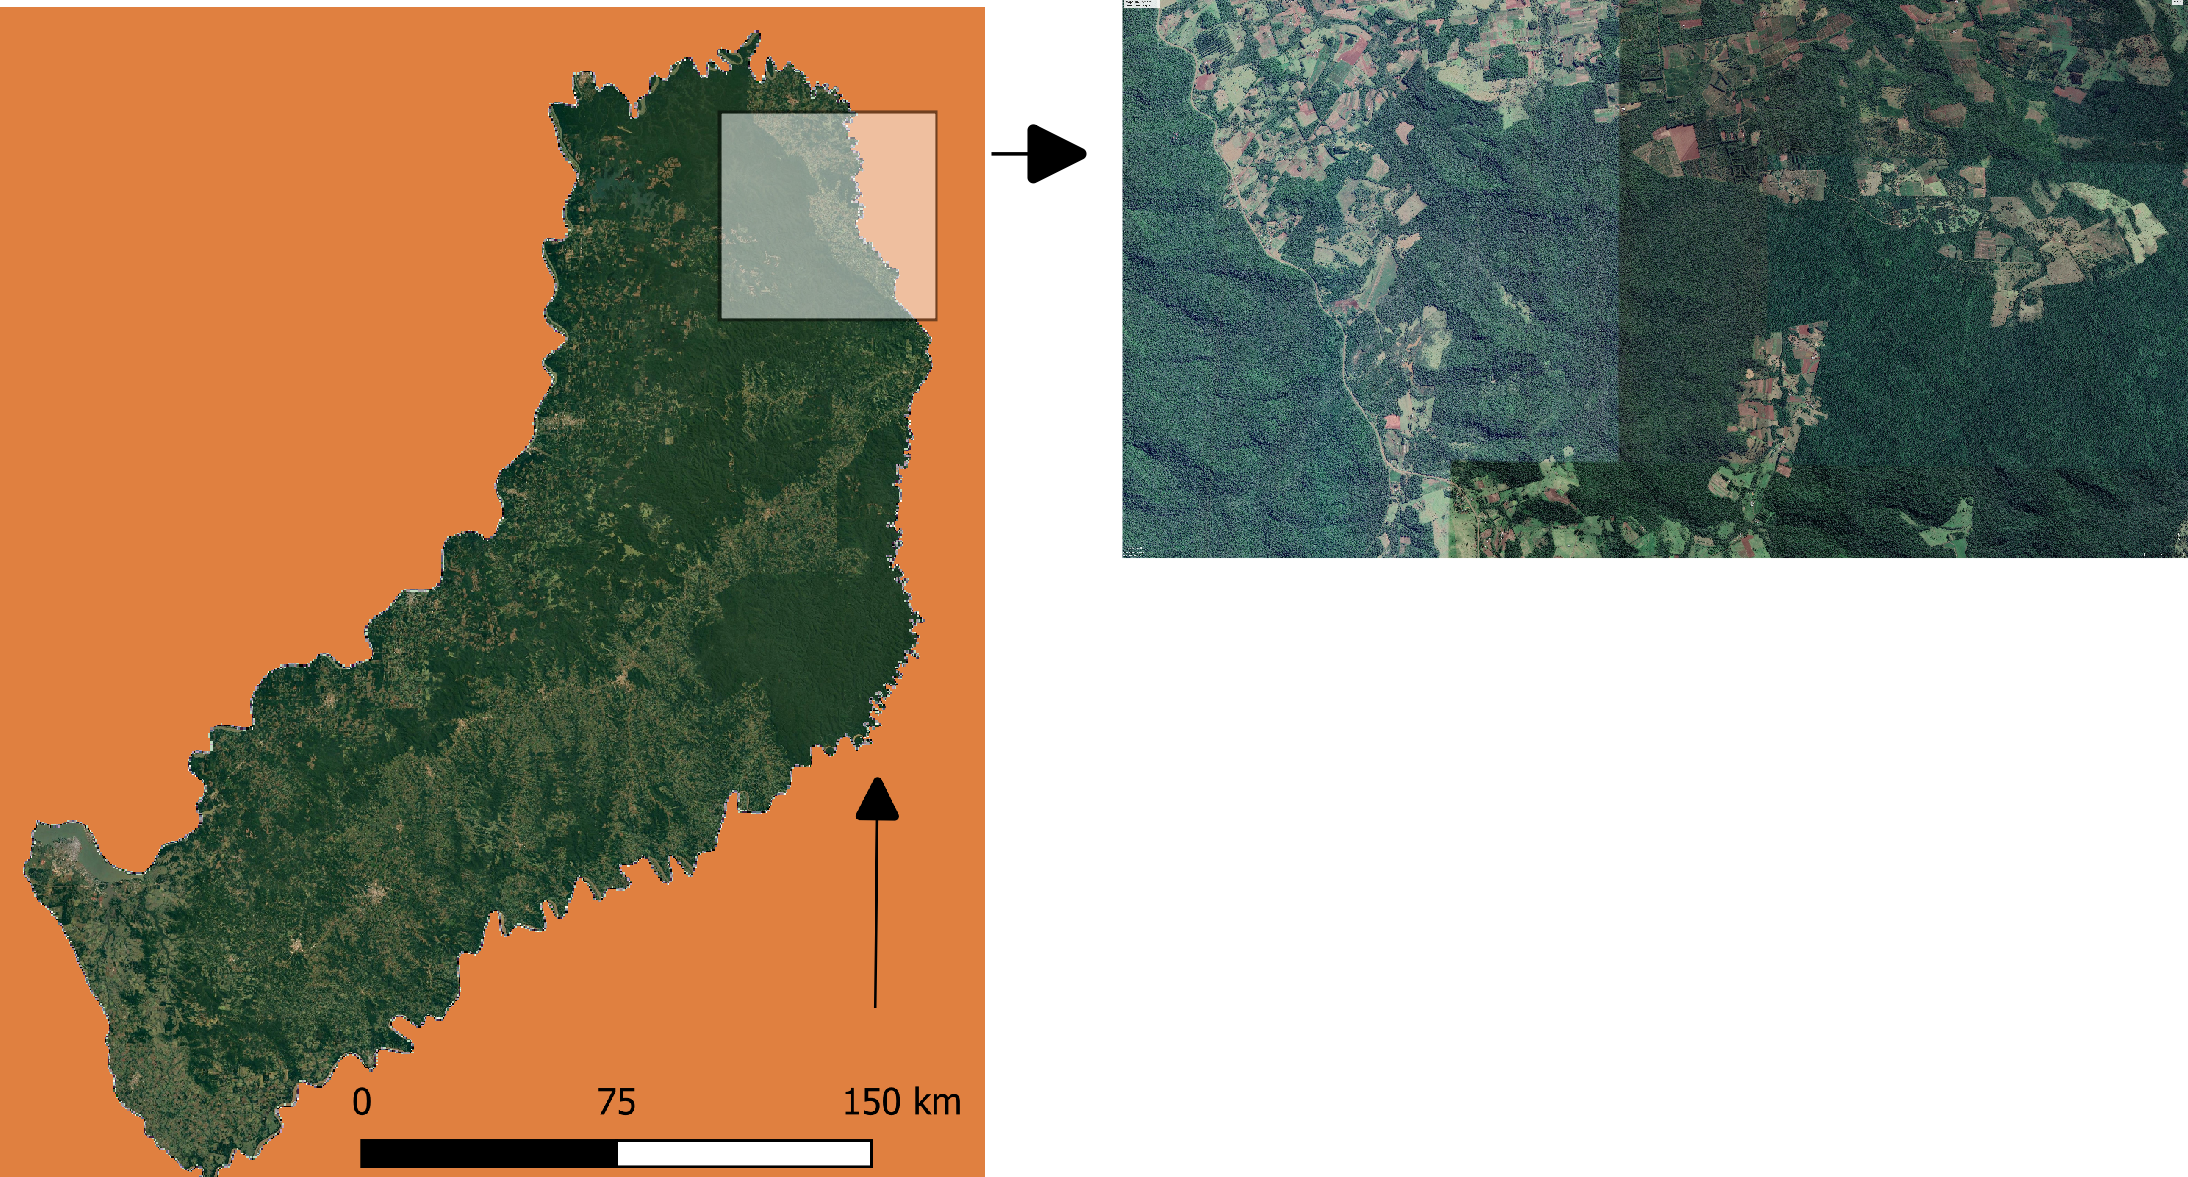
\includegraphics[width=30mm]{Imagenes/San Sebastian.png}}\\ 
\textbf{Administración} & Privada\\
        
        \textbf{Ubicación} & -25,857; -53,976 \\
         
        \textbf{Superficie} & 92 ha\\
\hline        
\end{tabular}

\label{San Sebastian}
\end{table}

La reserva San Sebastián de la Selva es una reserva privada de cien hectáreas, que contiene áreas de selva virgen y de selva en restauración. Está ubicada en la localidad de Comandante Andresito, al norte de la provincia de Misiones, sobre la ruta nacional 101, entre los parques Urugua-í y Foerster, contribuyendo a formar un corredor verde.
\subsubsection{Parque Provincial Cañadón de Profundidad}
\begin{table}[H]
\centering
\begin{tabular}{|c|c|c|}
\hline
 \textbf{Reserva} & Parque Provincial Cañadón de Profundidad &   \multirow{ 3}{*}{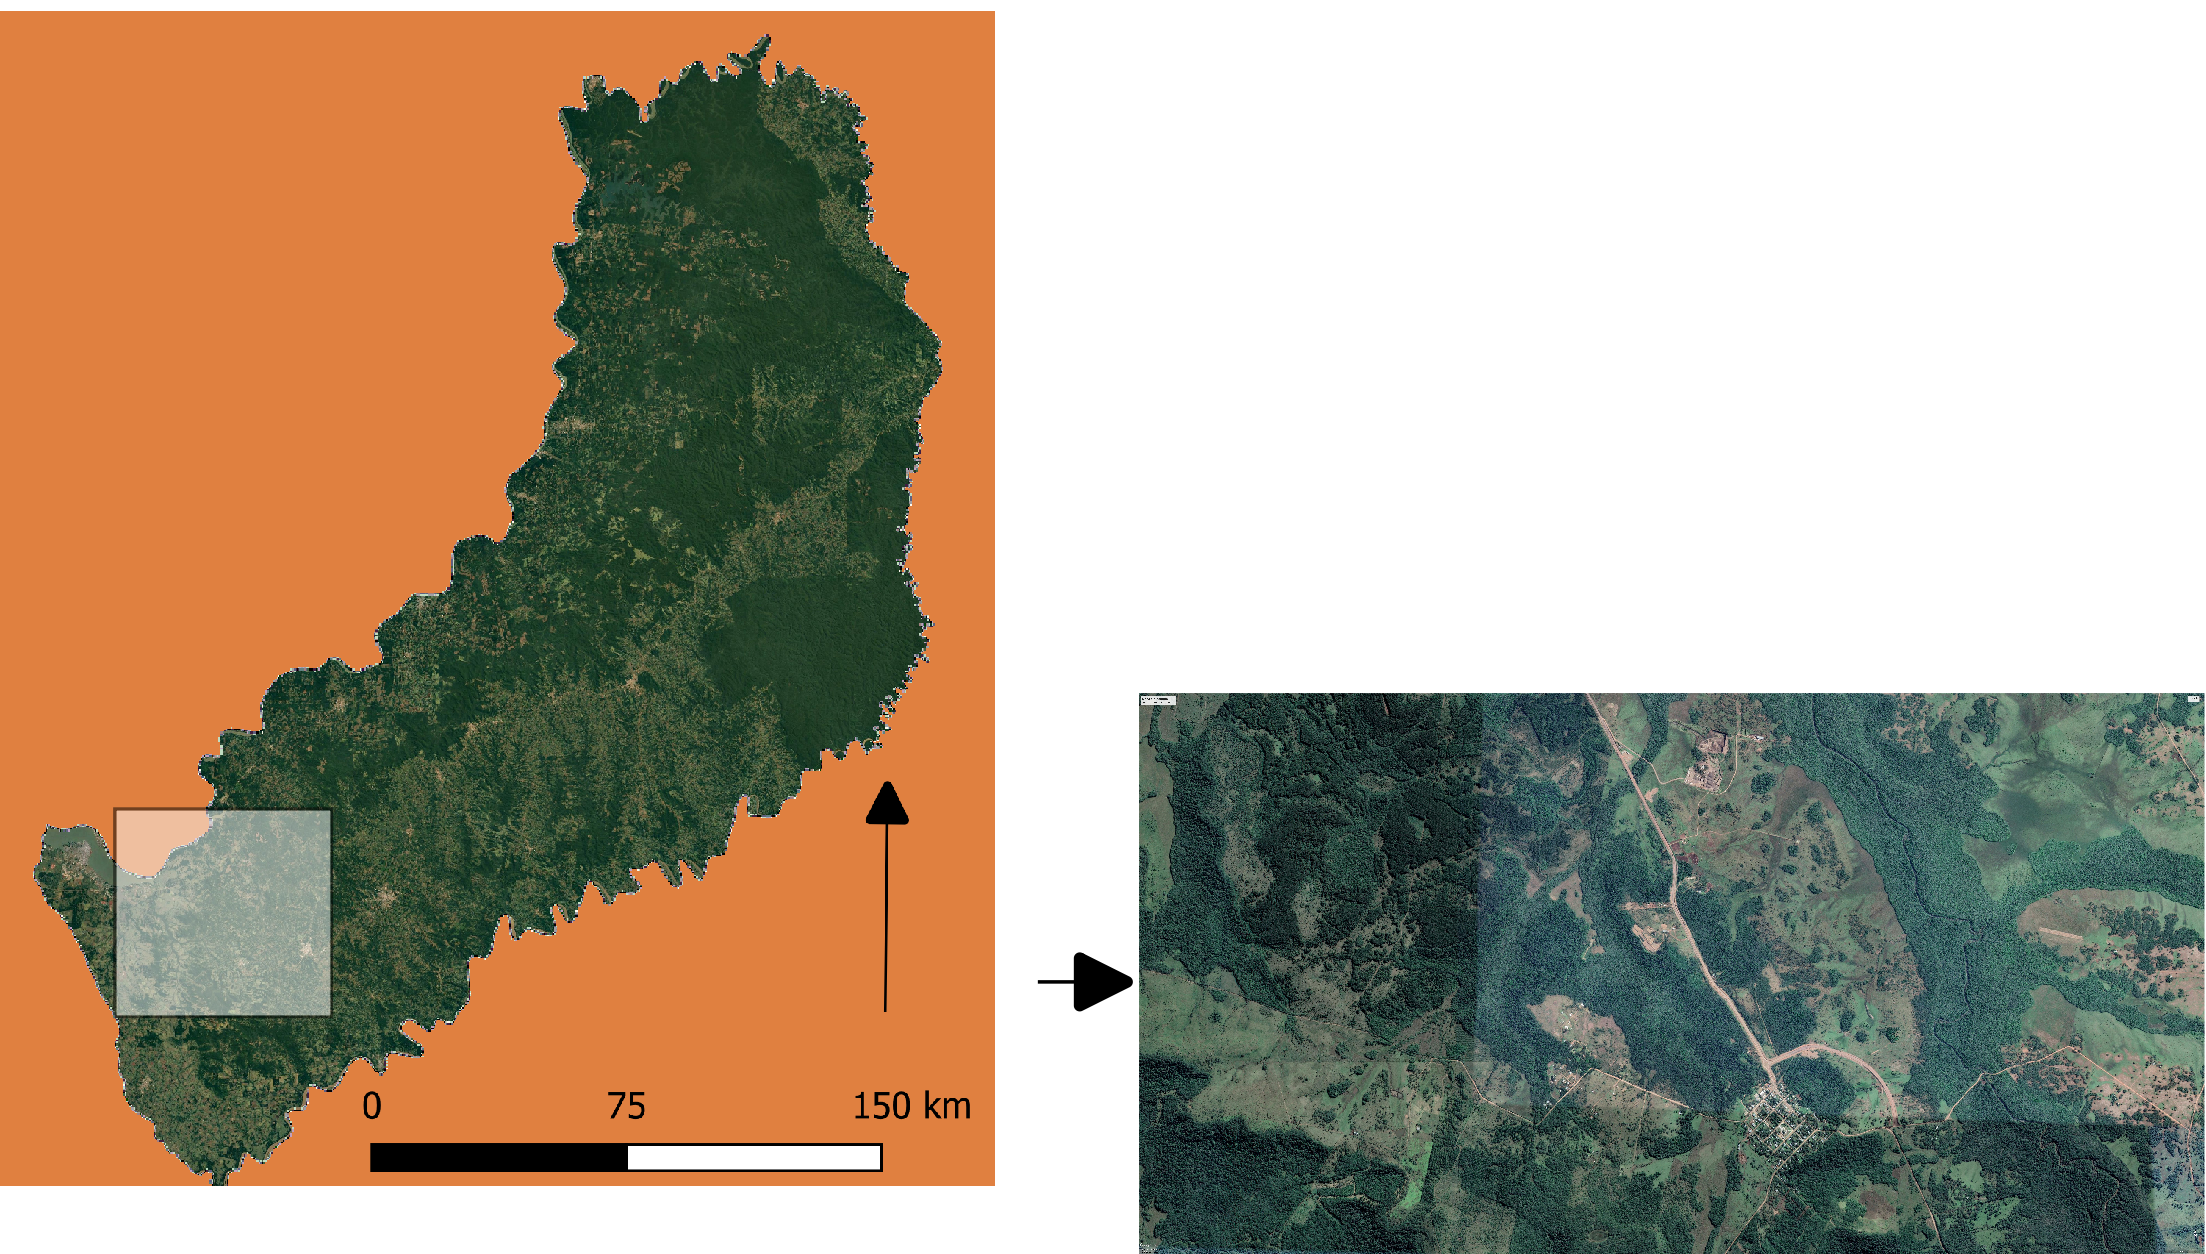
\includegraphics[width=30mm]{Imagenes/Profundidad.png}}\\ 
\textbf{Administración} & Pública\\
        
        \textbf{Ubicación} & -27,558; -55,702 \\
         
        \textbf{Superficie} & 19 ha\\
\hline        
\end{tabular}

\label{Profundidad}
\end{table}

La reserva provincial Cañadón de Profundidad es una pequeña reserva de alrededor de 20 ha ubicado en el departamento Candelaria, en cercanías de la ciudad de Posadas.

\subsection{Requerimientos y restricciones} \label{Metodo calculo relevamiento}
Para llevar adelante el relevamiento de las áreas forestales hay que tener en cuenta los requerimientos en el tiempo y en el equipamiento, así como las restricciones que imponen las regulaciones legales y condiciones geográficas y meteorológicas. Dependiendo de cuán grande sea el área a relevar, puede resultar más conveniente alguna de las plataformas de sensado remoto que otra. El criterio que debe ponderarse está basado en cálculos de tiempo, de costos operacionales y de disponibilidad. Para distintos escenarios, reservas grandes de miles de hectáreas de extensión o pequeñas reservas privadas de pocas decenas o centenas de hectáreas, los cálculos arrojarán resultados diferentes.
\subsubsection{Cálculo de tiempo}
Para poder comparar entre las diferentes opciones de plataformas para captura de imágenes aeroespaciales, es necesario conocer determinados parámetros de cada una. Un parámetro es el tiempo necesario para captura de imágenes de un determinado área. El costo asociado a la operación de captura de imágenes es otro parámetro a ser tenido en cuenta. Finalmente hay otros parámetros sobre los que las opciones pueden soportarse. Uno es el porcentaje de área útil sobre área total relevada. Otro parámetro es el espacio de almacenamiento requerido.
Si se comparan imágenes obtenidas por satélites contra aquellas obtenidas por aeronaves tripuladas o VANT, resulta evidente que aquellas cubren una extensión mayor, por lo que una sola captura puede exceder en mucho la zona de interés. 
Para hallar el factor de escala $m_b$, relacionamos la altura de vuelo $H_g$ con la distancia focal
de la cámara $f$ mediante la ecuación \ref{escala} \cite{linder_digital_2016}:
 %%%%%%%%%%%%%%%%%%%%%%%%%%%%%%%%%%%%%% ECUACIÓN %%%%%%%%%%%%%%%%%%%%%%%%%%%%%%%%%%%%%%%%%%%%%%%%%%%%%%%%%
\\
\begin{equation}
	m_b=\frac{H_g}{f},\label{escala}
\end{equation}
\\
%%%%%%%%%%%%%%%%%%%%%%%%%%%%%%%%%%%%%%%%%%%%%%%%%%%%%%%%%%%%%%%%%%%%%%%%%%%%%%%%%%%%%%%%%%%%%%%%%%%%%%%%%
Para hallar cualquier distancia en la superficie real a partir de la fotografía, se aplica la relación de escala:
 %%%%%%%%%%%%%%%%%%%%%%%%%%%%%%%%%%%%%% ECUACIÓN %%%%%%%%%%%%%%%%%%%%%%%%%%%%%%%%%%%%%%%%%%%%%%%%%%%%%%%%%
\\
\begin{equation}
	S=\frac{S'H_g}{f},\label{escala1}
\end{equation}
\\
%%%%%%%%%%%%%%%%%%%%%%%%%%%%%%%%%%%%%%%%%%%%%%%%%%%%%%%%%%%%%%%%%%%%%%%%%%%%%%%%%%%%%%%%%%%%%%%%%%%%%%%%%
donde $S$ es la distancia en la superficie real, $S'$ es la distancia en la imagen.
En un relevamiento fotogramétrico de áreas urbanas o cultivos, el solapamiento longitudinal suele ser de un promedio de 60\%, sin embargo,  mientras que el solapamiento lateral suele ser de 25\% [4], sin embargo, en zonas de selva densa se recomienda que sea mayor al 80\% para ambos solapamientos. La distancia longitudinal $B$ entre dos fotografías consecutivas (línea de base) se halla en función al solapamiento longitudinal $p$, y se calcula según la ecuación (\ref{linea_de_base}).
 %%%%%%%%%%%%%%%%%%%%%%%%%%%%%%%%%%%%%% ECUACIÓN %%%%%%%%%%%%%%%%%%%%%%%%%%%%%%%%%%%%%%%%%%%%%%%%%%%%%%%%%
\\
\begin{equation}
	B=S(1-\frac{p}{100}),\label{linea_de_base}
\end{equation}
\\
%%%%%%%%%%%%%%%%%%%%%%%%%%%%%%%%%%%%%%%%%%%%%%%%%%%%%%%%%%%%%%%%%%%%%%%%%%%%%%%%%%%%%%%%%%%%%%%%%%%%%%%%%
La distancia $a$ entre dos líneas de sobrevuelo adyacentes se define por el solapamiento lateral $q$.
  %%%%%%%%%%%%%%%%%%%%%%%%%%%%%%%%%%%%%% ECUACIÓN %%%%%%%%%%%%%%%%%%%%%%%%%%%%%%%%%%%%%%%%%%%%%%%%%%%%%%%%%
\\
\begin{equation}
	a=S(1-\frac{q}{100}),\label{distancia_adyacente}
\end{equation}
\\
%%%%%%%%%%%%%%%%%%%%%%%%%%%%%%%%%%%%%%%%%%%%%%%%%%%%%%%%%%%%%%%%%%%%%%%%%%%%%%%%%%%%%%%%%%%%%%%%%%%%%%%%%
Cuando se trata de un vuelo para realizar fotografías aéreas, ya sea tripulado o no, partiendo de conocer el área de interés, sus dimensiones, es posible definir las trayectorias de vuelo. De esta forma el relevamiento fotográfico aéreo se asemeja a una especie de "barrido", con varias líneas adyacentes. A lo largo de una línea se capturan imágenes de modo que se superpongan como mínimo en un 80\% dos fotografías consecutivas. Al final de cada línea la aeronave ejecuta un giro de 180º respecto al eje nadir-cenit de modo que al finalizar el giro su proa apunte en dirección contraria a la que tenía antes de iniciar el giro. Así inicia el recorrido de una nueva línea de vuelo, la cual es paralela a la anterior, separada una distancia que garantice un solapamiento mínimo de 25\% de imágenes en líneas de vuelo adyacentes. A partir de todo ello puede establecerse la cuenta de imágenes totales que cubran toda el área, así como el tiempo necesario para llevarlo a cabo. De esto también se obtiene el espacio de almacenamiento en memoria requerido.
La cantidad de imágenes por línea de vuelo $I_lv$ se puede conocer dada la longitud de la línea de vuelo $L_v$ y la línea de base $B$, mediante la ecuación (\ref{cantidad_imagenes}):
  %%%%%%%%%%%%%%%%%%%%%%%%%%%%%%%%%%%%%% ECUACIÓN %%%%%%%%%%%%%%%%%%%%%%%%%%%%%%%%%%%%%%%%%%%%%%%%%%%%%%%%%
\\
\begin{equation}
	I_{lv}=\frac{L_v}{B},\label{cantidad_imagenes}
\end{equation}
\\
%%%%%%%%%%%%%%%%%%%%%%%%%%%%%%%%%%%%%%%%%%%%%%%%%%%%%%%%%%%%%%%%%%%%%%%%%%%%%%%%%%%%%%%%%%%%%%%%%%%%%%%%%
Multiplicando el resultado de la ecuación \ref{cantidad_imagenes} por la cantidad de líneas de vuelo $N_{lv}$ se obtiene la cantidad total de imágenes $I_t$ para toda el área relevada:
  %%%%%%%%%%%%%%%%%%%%%%%%%%%%%%%%%%%%%% ECUACIÓN %%%%%%%%%%%%%%%%%%%%%%%%%%%%%%%%%%%%%%%%%%%%%%%%%%%%%%%%%
\\
\begin{equation}
	I_t={I_{lv}}{N_{Lv}},\label{cantidad_total_imagenes}
\end{equation}
\\
%%%%%%%%%%%%%%%%%%%%%%%%%%%%%%%%%%%%%%%%%%%%%%%%%%%%%%%%%%%%%%%%%%%%%%%%%%%%%%%%%%%%%%%%%%%%%%%%%%%%%%%%%
El espacio de almacenamiento necesario de cada imagen $M_i$ está determinado por las características de los sensores, la cantidad de píxeles $Px$, cantidad de bandas espectrales $B_e$, la profundidad en bits de cada canal $Pb$:
  %%%%%%%%%%%%%%%%%%%%%%%%%%%%%%%%%%%%%% ECUACIÓN %%%%%%%%%%%%%%%%%%%%%%%%%%%%%%%%%%%%%%%%%%%%%%%%%%%%%%%%%
\\
\begin{equation}
	M_i={Px}{B_e}{P_b},\label{memoria}
\end{equation}
\\
%%%%%%%%%%%%%%%%%%%%%%%%%%%%%%%%%%%%%%%%%%%%%%%%%%%%%%%%%%%%%%%%%%%%%%%%%%%%%%%%%%%%%%%%%%%%%%%%%%%%%%%%%
Multiplicando el resultado de la ecuación \ref{memoria} por la cantidad total de imágenes $I_t$ se obtiene la cantidad de memoria total para almacenar todas las imágenes del relevamiento del área:
  %%%%%%%%%%%%%%%%%%%%%%%%%%%%%%%%%%%%%% ECUACIÓN %%%%%%%%%%%%%%%%%%%%%%%%%%%%%%%%%%%%%%%%%%%%%%%%%%%%%%%%%
\\
\begin{equation}
	M_t={M_i}{I_t},\label{memoria_total}
\end{equation}
\\
%%%%%%%%%%%%%%%%%%%%%%%%%%%%%%%%%%%%%%%%%%%%%%%%%%%%%%%%%%%%%%%%%%%%%%%%%%%%%%%%%%%%%%%%%%%%%%%%%%%%%%%%%
En un relevamiento fotográfico aéreo, ya sea tripulado o no, el tiempo que lleva realizar el procedimiento está determinado por la velocidad de desplazamiento de la plataforma $V_p$, y la longitud total de vuelo $L_vT$. 
En el caso de que el área relevada sea un rectángulo, $L_v$ podría fácilmente calcularse conociendo uno de los lados del rectángulo, que sería la longitud de línea de vuelo $L_v$, multiplicando por la cantidad de líneas de vuelo $N_{lv}$:
 %%%%%%%%%%%%%%%%%%%%%%%%%%%%%%%%%%%%%% ECUACIÓN %%%%%%%%%%%%%%%%%%%%%%%%%%%%%%%%%%%%%%%%%%%%%%%%%%%%%%%%%
\\
\begin{equation}
	L_{vt}={L_v}{N_{lv}},\label{longitud_total}
\end{equation}
\\
%%%%%%%%%%%%%%%%%%%%%%%%%%%%%%%%%%%%%%%%%%%%%%%%%%%%%%%%%%%%%%%%%%%%%%%%%%%%%%%%%%%%%%%%%%%%%%%%%%%%%%%%%
Dividiendo el resultado de \ref{longitud_total} por la velocidad de desplazamiento $V_p$ se obtiene el tiempo que tardará en completar el recorrido. Para ser rigurosos, debería añadirse el tiempo que lleva trasladarse a la plataforma desde la base de operaciones (el aeródromo en el caso de aeronaves tripuladas) hasta el inicio del recorrido, y desde el punto final en retorno a la base.
Conociendo el tiempo total que le lleva a la plataforma aérea completar el recorrido, se puede tomar como base para el cálculo de costo de obtención de las imágenes para el caso de aeronaves tripuladas y VANT, el cual suele ir expresado en montos de dinero por unidad de tiempo, generalmente por hora. \\
Obtener los datos y características técnicas de los sensores no es tarea sencilla. La información que suele figurar en los sitios web de los fabricantes o en los manuales, no suele ser la que se necesita para calcular. Por ejemplo la distancia focal no suele ser un dato que aparezca en la lista de especificaciones. Puede obtenerse de los metadatos asociados a una imagen que ha sido capturada con ese sensor.
Del mismo modo tampoco resulta sencillo obtener información sobre las tarifas de vuelos de relevamiento aéreo, ya sea tripulado o no. La información disponible es vaga y escueta, por ejemplo en respuesta a una consulta han informado que la hora de vuelo tripulado es de 240 dólares estadounidenses si se toma como base el dólar oficial (cotizado en 55 mil pesos argentinos, mayo 2023), y la de VANT es de 195 dólares estadounidenses (cotizado en 45 mil pesos argentinos, mayo 2023). Según otras consultas, el costo de hora de vuelo de aviones tripulados es de alrededor de cien dólares estadounidenses \footnote{Las consultas fueron realizadas a distintos referentes de la actividad aeronáutica}.
\subsubsection{Carga útil - cámaras fotográficas}
Los que se pueden seleccionar con mayor grado de libertad son los que están relacionados con el hardware asociado a la tarea, como es el sensor de la cámara, o las características de funcionamiento de la aeronave no tripulada. Una cámara con mayor resolución demandará mayor espacio de almacenamiento. Asimismo si se trata de sensores ópticos en el rango del espectro visible, la posibilidad de operar se limitará a las horas diurnas. No así si se trata de sensores que trabajan en otro rango de longitudes de onda, como los infrarrojos, o sensores activos, como LiDAR.
\subsubsection{Marco regulatorio} %Marco teórico
Las imágenes utilizadas en el presente trabajo son de libre disponibilidad (Google, Bing, banco de imágenes satelitales de la NASA, ESA...). Las que se obtuvieron por medios propios se han hecho en lugares públicos previniendo la fotografía de personas y dentro del marco que regula las actividades con VANT. 
\subsubsection{Almacenamiento necesario} %fusionar con Hardware
Dependiendo de la resolución espacial y espectral de las imágenes, los requerimientos de almacenamiento aumentarán en proporción a las mismas. Por ejemplo, para relevar completamente un área de la extensión de la reserva Biósfera Yaboty, con una resolución espacial de 3 cm/pixel, las casi seis millones y medio de fotografías en RGB, con 5 Megapíxeles por cada una, con una profundidad de color de 8 bit por canal necesitarían un espacio de almacenamiento de alrededor de 7,5 Terabytes.

\section{Procesamiento de imágenes} \label{Metodo bloque 2}


\subsection{Procesamiento con filtro homomórfico} \label{Metodo homomorfico}
Tomando como base el modelo de iluminación de Stockham para descomponer partes iluminadas de sombreadas, adoptando el concepto de frecuencia espacial, se implementó un procedimiento que incluía una etapa de filtrado homomórfico seguida de una etapa de aplicación de lógica difusa para discriminar sombras en imágenes aéreas de porciones de selva. El diagrama de flujo del procesamiento se describe en la figura \ref{flowchart_homomorfico}.
La imagen se modela como el producto de una componente de iluminación y otra de reflexión, que depende de las características del objeto iluminado. 
La ecuación que representa al filtro es \ref{filtro homomorfico}
%%%%%%%%%%%%%%%%%%%%%%%%%%%%%%%%%%%%%% ECUACIÓN %%%%%%%%%%%%%%%%%%%%%%%%%%%%%%%%%%%%%%%%%%%%%%%%%%%%%%%%%
\\
\begin{equation}
	H(u,v)=1-((\gamma_H-\gamma_L)(1-e^{\frac{-cD^L(u,v)}{D^L_0}}+\gamma_L),\label{filtro homomorfico}
\end{equation}
\\
%%%%%%%%%%%%%%%%%%%%%%%%%%%%%%%%%%%%%%%%%%%%%%%%%%%%%%%%%%%%%%%%%%%%%%%%%%%%%%%%%%%%%%%%%%%%%%%%%%%%%%%%%  
\begin{figure}[h!]
    \centering
    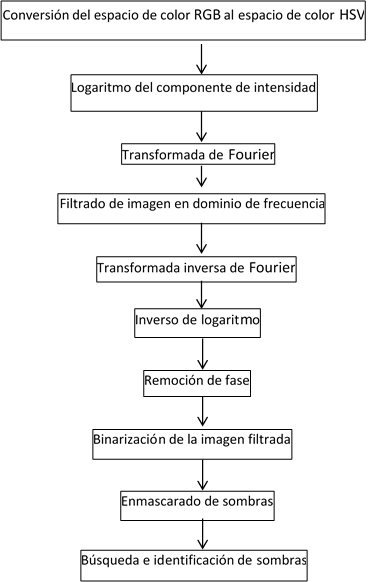
\includegraphics[width=0.5\textwidth]{Imagenes/Homomorfico/flowchart.png}
     \hfill
     \caption{Diagrama de flujo del procesamiento homomórfico}
    \label{flowchart_homomorfico}
\end{figure}

donde $D_0$ es la frecuencia de corte, $c$ controla la forma y pendiente del filtro en la región de transición entre $\gamma_L$ y $\gamma_H$. $D(u,v)$ es la distancia al origen del plano de frecuencias.

Las imágenes a ser analizadas son imágenes satelitales obtenidas desde el sitio web Bing, de distintas reservas de bosque nativo, tanto públicas como privadas, %\color{red}\textbf{(poner en referencia de la dirección web del maps)}\color{black}. \\ % Paranay -26.701277, -54.759434
en los que se supone mayor presencia de especies de árboles de interés para el presente trabajo. 
\subsubsection{Selección automática de regiones sombreadas usando método de recorrido de ventana} \label{metod_homo_ventana}
En un primer paso se realizó la conversión de la imagen de color rojo, verde y azul (RGB) a la representación matiz, saturación e intensidad (HSI), trabajando sobre la componente de intensidad. La componente de intensidad se obtiene sumando los tres canales rojo, verde y azul y dividiendo por tres (ecuación \ref{RGB-HSI}). 
%%%%%%%%%%%%%%%%%%%%%%%%%%%%%%%%%%%%%% ECUACIÓN %%%%%%%%%%%%%%%%%%%%%%%%%%%%%%%%%%%%%%%%%%%%%%%%%%%%%%%%%
\\
\begin{equation}
	I=\frac{R+G+B}{3},\label{RGB-HSI}
\end{equation}
\\
donde $I$ es el valor de intensidad, $R$, $G$ y $B$ son los valores respectivos de las bandas roja, verde y azul.
%%%%%%%%%%%%%%%%%%%%%%%%%%%%%%%%%%%%%%%%%%%%%%%%%%%%%%%%%%%%%%%%%%%%%%%%%%%%%%%%%%%%%%%%%%%%%%%%%%%%%%%%%  
En un paso siguiente se aplicó el logaritmo a la componente de intensidad de la imagen y seguidamente se obtuvo la transformada de Fourier de la misma, para poder procesar con el filtro de sombras, expresado en la ecuación \ref{filtro homomorfico}. Se multiplicó la matriz de la imagen por la matriz que representa al filtro y luego, al resultado se le aplicó la transformada inversa de Fourier, la función inversa de logaritmo y la remoción de fase, tomando el módulo del número complejo, todo en orden sucesivo. 
Posteriormente se binarizó la imagen filtrada fijando un valor de umbral dentro de una escala de 0 a 1 en la que el valor 1 es blanco y 0 es negro, de modo que a los píxeles con valor de intensidad menor al umbral se les asignó el valor cero, y a los que superaban el valor umbral se les asignaba el valor 1. La imagen de salida del filtro de sombras constituye así una máscara que presenta a las sombras resaltadas con píxeles de intensidad blancos. En la siguiente etapa del algoritmo se implementa una selección de las regiones que corresponden a sombras en la imagen, donde por medio de una ventana cuadrada que recorre todo el ancho y largo de la imagen se evalúan las distintas sombras por su tamaño, descartándose las que son muy pequeñas de acuerdo a un parámetro establecido. Finalmente se obtiene una máscara binaria que contiene las demarcaciones de sombras en la imagen.

\subsubsection{Selección automática de regiones sombreadas usando método de inferencia difusa a partir del filtrado homomórfico} \label{metod_homo_fuzzy}
Partiendo de la imagen procesada con filtro homomórfico, se efectuó la selección de las sombras binarizadas mediante técnicas de lógica difusa, en dos etapas (ver figura \ref{flowchart_homofuzzy}. \\

\begin{figure}[h!]
    \centering
    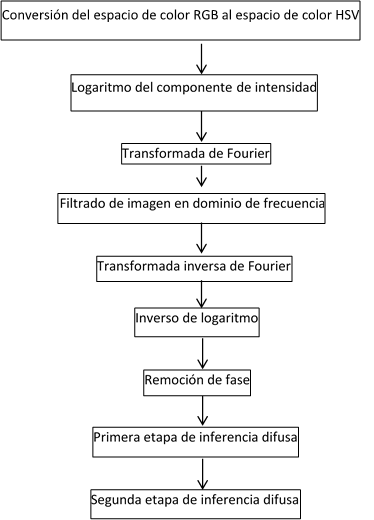
\includegraphics[width=0.5\textwidth]{Imagenes/Homomorfico/flowchart_fuzzy.png}
     \hfill
     \caption{Diagrama de flujo del procesamiento homomórfico con sistema de inferencia difuso}
    \label{flowchart_homofuzzy}
\end{figure}

En la primera implementando un sistema de inferencia difusa por el método Sugeno, mediante el cual se discriminaban los píxeles de determinada intensidad, que constituía la variable de entrada, estableciendo una salida según dos funciones de membresía trapezoidales, una correspondiente a píxeles "claros" y otra a "oscuros" (ver figura \ref{sug1}). La segunda etapa de inferencia difusa, también con el método Sugeno, implicaba dos variables de entrada, área e intensidad promedio. A cada variable se le asignaron funciones de membresía, tres en el caso de área, de forma trapezoidal, y dos en el caso de la variable intensidad promedio, de forma triangular (ver figura \ref{sug2}). La salida del sistema es una máscara binaria con las regiones de sombra designadas con píxeles blancos. 

%%%%%%%%%%%%%%%%%%%%%%%%%%%%%%%%%%%%%%%%%%%%%%%%%%%%%%%%%%%%%%%%%%%%%%%%%%%%%%%%%%%%%%%%%%%%%%%%%%%%%%%%%  
\begin{figure}[h!]
    \centering
    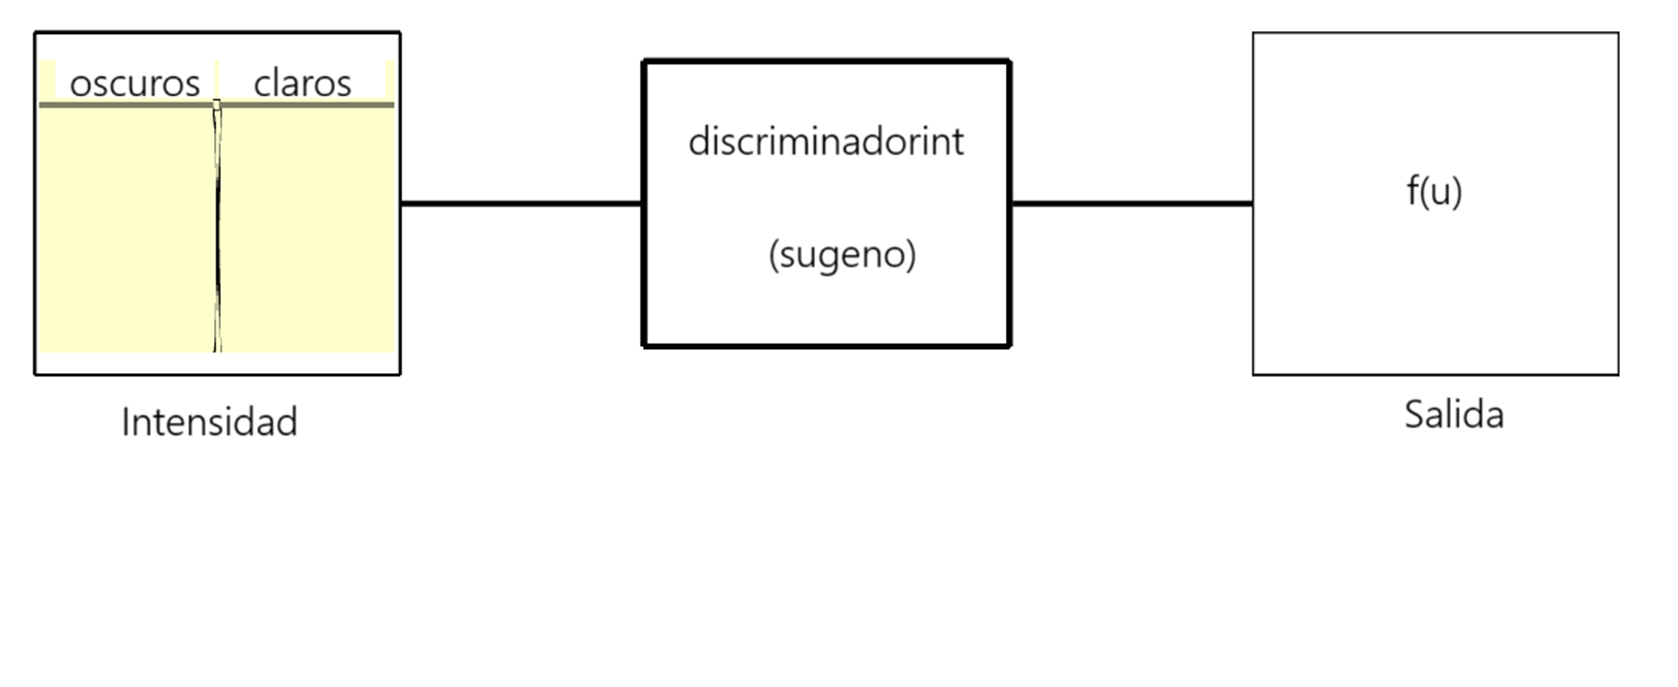
\includegraphics[width=0.5\textwidth]{Imagenes/Homomorfico/sugeno1.png}
     \hfill
     \caption{Esquema del sistema de inferencia difusa de la primera etapa}
    \label{sug1}
\end{figure}
%%%%%%%%%%%%%%%%%%%%%%%%%%%%%%%%%%%%%%%%%%%%%%%%%%%%%%%%%%%%%%%%%%%%%%%%%%%%%%%%%%%%%%%%%%%%%%%%%%%%%%%%%  
\begin{figure}[h!]
    \centering
    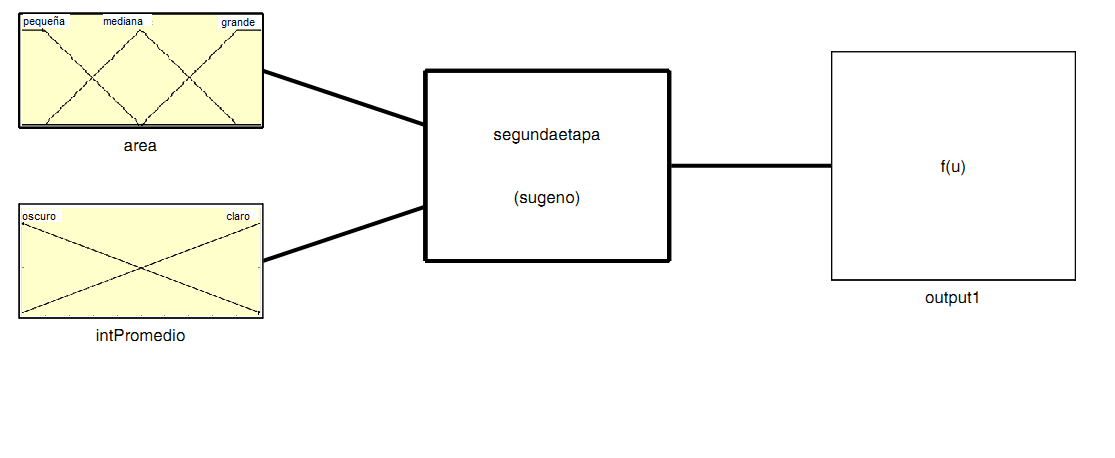
\includegraphics[width=0.5\textwidth]{Imagenes/Homomorfico/sugeno2.png}
     \hfill
     \caption{Esquema del sistema de inferencia difusa de la segunda etapa}
    \label{sug2}
\end{figure}

%Faltaría añadir una explicación de cómo se obtiene el error medio
\subsubsection{Estadísticos} 
El error medio se obtiene restando al conteo automático el conteo manual, dividiendo por la cantidad de imágenes analizadas, que en este caso fueron once.
La varianza se calcula mediante la fórmula expresada en la ecuación \ref{varianza}.
%%%%%%%%%%%%%%%%%%%%%%%%%%%%%%%%%%%%%% ECUACIÓN %%%%%%%%%%%%%%%%%%%%%%%%%%%%%%%%%%%%%%%%%%%%%%%%%%%%%%%%%
\\
\begin{equation}
	\sigma_{e} ^2=\frac{\sum (x_{i}-\overline{x})^2}{n},\label{varianza}
\end{equation}
\\
siendo $x_i$ el valor de cada conteo automático de cada una de las $n$ imágenes analizadas, y $\overline{x}$ es el valor de conteo manual.
%%%%%%%%%%%%%%%%%%%%%%%%%%%%%%%%%%%%%%%%%%%%%%%%%%%%%%%%%%%%%%%%%%%%%%%%%%%%%%%%%%%%%%%%%%%%%%%%%%%%%%%%%  
El desvío estándar se obtiene de la raíz cuadrada de la varianza (ecuación \ref{desvio}.
%%%%%%%%%%%%%%%%%%%%%%%%%%%%%%%%%%%%%% ECUACIÓN %%%%%%%%%%%%%%%%%%%%%%%%%%%%%%%%%%%%%%%%%%%%%%%%%%%%%%%%%
\\
\begin{equation}
	\sigma_{e}=\sqrt{\frac{\sum (x_{i}-\overline{x})^2}{n}},\label{desvio}
\end{equation}
\\
\subsection{Procesamiento morfológico} %Ferreira, Wagner...

El tratamiento automático de clasificación de especies arbóreas a partir de imágenes requiere de un conjunto de habilidades informáticas que van desde la manipulación el tratamiento de las imágenes hasta el entrenamiento de modelos de aprendizaje automático. Para obtener una aceptable clasificación de copas es necesario realizar procesamiento a la imagen aprovechando las características de textura y contraste que ésta exhibe. Los algoritmos matemáticos desarrollados en este trabajo posibilitan una adecuada segmentación de las copas individuales del dosel y capa emergente de la Selva Atlántica, lo que consecuentemente habilita en otro nivel la clasificación por especies. 
Para obtener el segmentado se toma como punto de partida la imagen aérea en escala de grises, ya que se enfoca en los diferentes contrastes y texturas existentes entre el área de copas y el espacio entre ellas. Corresponde hacer una primer etapa de identificación gruesa entre copas y bordes, luego se homogeneiza el interior de las copas para eliminar huecos. La imagen es tratada matemáticamente como una matriz donde cada elemento es un píxel, cuyo valor se relaciona con la intensidad correspondiente al espacio de color HSI. Esta matriz es pasible de manipulación matemática, de modo que permite aplicarse filtros varios, algoritmos de procesamiento morfológicos, que permiten resaltar estructuras internas de la imagen, facilitando esto la segmentación de copas. Se aplica un criterio de distinción de tamaño de copas grandes y chicas, partiendo desde la resolución espacial de la imagen, definiendo aquellas grandes como las que superan el radio de tres píxeles. Diferentes algoritmos se aplican de forma secuenciada, procesando sobre los resultados de cada paso anterior. De modo que intervienen algoritmos de homogeneización como el filtro \textit{RollingBall} y el filtrado \textit{top-bottom-hat} basado en operadores morfológicos de apertura y clausura. En cada etapa se definen parámetros que se ajustan según las condiciones
de la imagen, algunos de los cuales se obtienen por medio de herramientas de estadística (promedio, percentiles, etc.). Estos parámetros son tenidos en cuenta para definir umbrales de decisión. A los fines de visualizar el comportamiento de los algoritmos y la influencia de estos parámetros, se condujo una evaluación tipo \textit{gridsearch} en la que se definió un rango para cada parámetro y se expuso el resultado correspondiente. A continuación, se describe en detalle cada etapa de procesamiento, según lo ilustrado en la Figura \ref{flowchart_morfologico}. 

Para el diagrama de bloques:

1. Preprocesamiento\\
2. Eliminación de áreas sin sombra\\
3. Primera identificación de objetos oscuros\\
4. Relleno de sombras en copas\\
5. Identificación y relleno de huecos en grandes copas\\
6. Segunda identificación de objetos oscuros\\
7. Búsqueda de pequeños huecos en grandes copas\\
8. Homogenización de escala de grises en grandes árboles\\
9. Extracción de copas de segmentación\\
10.  Delineación de copas individuales\\

\begin{figure}[h!]
    \centering
    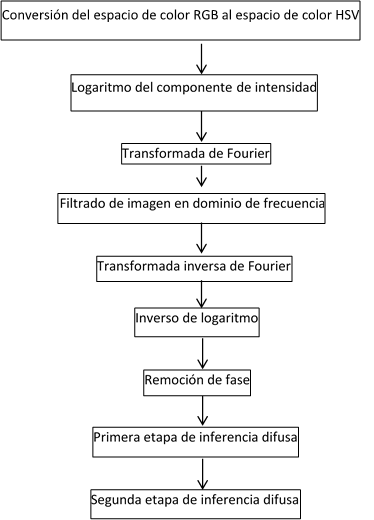
\includegraphics[width=0.5\textwidth]{Imagenes/Homomorfico/flowchart_fuzzy.png}
     \hfill
     \caption{Diagrama de flujo del procesamiento morfologico}
    \label{flowchart_morfologico}
\end{figure}


\subsubsection{Preprocesamiento y eliminación de áreas sin sombra}
La imagen es procesada en escala de grises, para ello se parte del formato original HSL (\textit{Hue}, \textit{Saturation}, \textit{Luminosity}) y se extrae solamente la componente de luminosidad, en la cual el valor de cada pixel varía en un rango entre 0 y 1, en el que los valores más altos corresponden a áreas más brillantes. También la imagen es recortada seleccionando las áreas de interés (las que contienen sombras).
\subsubsection{Primera identificación de objetos oscuros}
Una primera identificación de objetos oscuros se logra a partir de definir a los píxeles de la imagen que tienen un valor menor que la media en la distribución de grises.
\subsubsection{Relleno de sombras en copas}
Este paso es para "suavizar" la textura de las copas de los árboles, rellenando los espacios de sombras.
Si se invierte los valores de los píxeles de la imagen y se le suma el máximo valor de la escala de grises, se obtiene un equivalente a una imagen negativa. Luego se aplica un filtro \textit{Rolling Ball} con radio de tres píxeles. La imagen resultante se vuelve a invertir, quedando como resultado un área de píxeles homogéneo.
\subsubsection{Identificación y relleno de huecos en grandes copas}
Según la resolución espacial de la imagen utilizada, una copa de árbol de 7,5 m de diámetro abarca 15 píxeles. Se lleva a cabo una transformación top hat, con un elemento estructurante circular de diámetro de 15 píxeles. Se obtiene entonces una máscara binaria que contiene solamente copas grandes (mayores a 7,5 metros de diámetro).
\subsubsection{ Segunda identificación de objetos oscuros}
Se asume que la mayoría de los píxeles oscuros dentro de las copas de los árboles fueron removidos. Se realiza entonces una segunda identificación de píxeles oscuros, definidos como aquellos menores al 99º percentil de distribuciones en huecos.
\subsubsection{Búsqueda de pequeños huecos en grandes copas}
En las copas grandes existen áreas de huecos o sombras que a los efectos de facilitar la tarea de conteo de copas, es conveniente rellenarlos. Para realizarlo se analiza en una ventana de 7 por 7 píxeles la ocurrencia de valores distintos de cero alrededor de cada píxel. Estos tienen una distribución bimodal, donde los huecos en las copas son aquellos cuyos valores están por encima del 75º percentil. Al finalizar la etapa se identifican tres clases de píxel: los que corresponden a sombras entre árboles, los no sombreados en copas y los que son sombras en las copas. Se constituye una máscara binaria asignando 0 para píxeles fuera de copas y 1 para píxeles dentro de copas.
\subsubsection{Homogeneización de escala de grises en grandes árboles}
Los píxeles de las copas grandes son rellenados con la media de los cuatro mayores valores en una ventana de 7 por 7 píxeles.
\subsubsection{Extracción de copas de segmentación}
Mediante un filtro top bottom se efectua la extracción de copas de diámetro mayor a 3 m, usando un elemento estructural de 6 por 6 píxeles. Luego se umbraliza la imagen con el valor del 0,001 percentil.
\subsubsection{Delineación de copas individuales}
En esta etapa se calcula la distancia entre valores cero y distinto de cero, es decir la distancia del píxel al borde de la copa. Por medio de una ventana cuadrada se calcula el máximo local, y se genera una dilatación que duplique el diámetro.





%\color{cyan} %color de texto con 70-80 % o más de avance
\subsection{Método del Índice Invariante de color} \label{Metodología IIC}
%\subsubsection{Metodología propuesta IIC}
Un método que da resultados interesantes en la detección de sombras es el que implementaba el cálculo del índice invariante de color (IIC). 
%Probando con distintos valores de umbral, se observó que el que producía resultados más satisfactorios era el que correspondía al 85º percentil de la distribución de los valores de IIC.
El punto de partida del método es la adquisición de imágenes aéreas. No hay requerimientos especiales, excepto que se den las condiciones para proyección de sombras. Se tomaron imágenes de un área representativa de la selva nativa en la provincia de Misiones, las cuales fueron capturadas desde un VANT que sobrevoló las áreas de interés. A los efectos de obtener imágenes con presencia de sombras, se estableció un adecuado rango temporal de captura de imágenes, en este caso de 3 a 4 pm. Las imágenes fueron adquiridas en el invierno meridional, en el mes de agosto, cuando la proyección de sombras es mayor debido a la posición relativa del sol. Se utilizó un dron Mini 2, del fabricante DJI, equipado con una cámara de 12 megapíxeles. La altura de vuelo sobre el terreno fue de 50 metros. la resolución espacial de las imágenes son de 3 cm/píxel.

En esta sección se describen los pasos del método de procesamiento necesarios para obtener la máscara automática de sombras de la imagen aérea. La figura \ref{diagrama_procesamiento} representa la secuencia de procesamiento.

\begin{figure}
    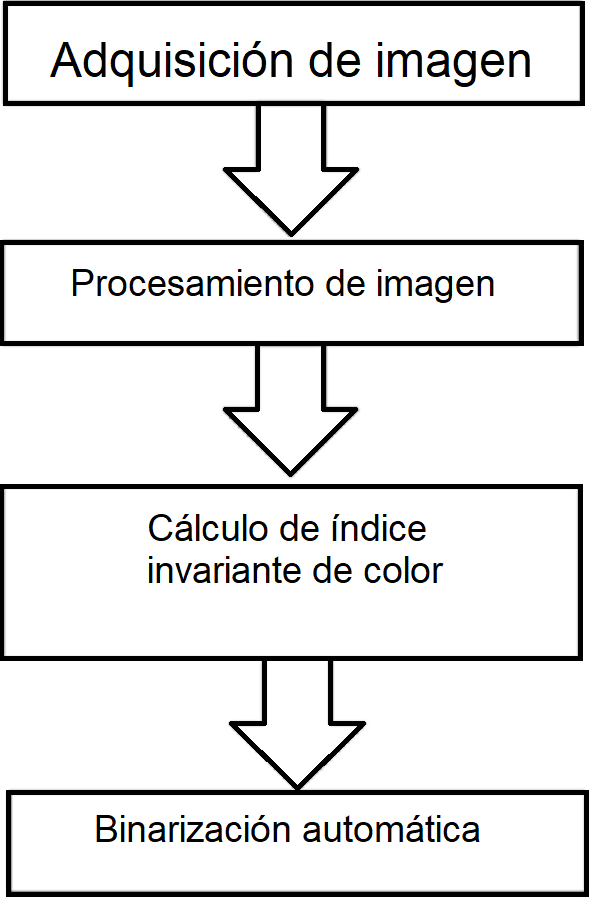
\includegraphics[width=0.3\textwidth]{Imagenes/flowchart.png}
     \hfill
     \caption{Diagrama del procesamiento}
    \label{diagrama_procesamiento}
\end{figure}

\subsubsection{Adquisición de la imagen}
Entre los pocos requerimientos en esta etapa se destaca que las condiciones de luz solar deben ser las apropiadas para generar proyecciones de sombra. Aquí se consideran imágenes representativas de un área de selva nativa en la provincia de Misiones, Argentina, que han sido capturadas mediante VANT sobrevolando porciones de selva en parques y reservas naturales, en las cuales habría presencia de ejemplares de árboles de interés. Para garantizar una mejor captura de imágenes con sombra, se seleccionó un intervalo de tiempo que abarca desde las 3 p.m. hasta las 4 p.m., que es cuando la posición relativa del sol facilita la proyección de sombras sobre el dosel. Las imágenes fueron capturadas durante el invierno meridional, específicamente en el mes de agosto, cuando las sombras proyectadas son mayores para ese horario. Se usó un VANT modelo Mini 2 del fabricante DJI, equipado con una cámara con resolución de 12 Megapíxeles. La altura de vuelo sobre el terreno fue de 50 metros, y el modo en que estuvo configurada la cámara era automático. Las imágens capturadas están en formato JPG con una resolución de 4000 x 2250 píxeles, con una resolución espacial de 3 cm/pixel aproximadamente. Para ejecutar el algoritmo se usó una computadora laptop común con un procesador Intel Core i5. En cuanto a los scripts, están basados en códigos de Octave. Se analizó un total de 19 imágenes.

\subsubsection{Preprocesamiento de imagen} 
Para facilitar el procesamiento y posterior análisis, las imágenes de los diferentes sitios deben ser recortadas par anormalizar el tamaó y ser filtradas para estandarizar algunos atributos.
\subsubsection{Cálculo de índice invariante de color}
Con base en imágenes filtradas RGB, el invariante de color $\Psi$ se calcula por medio de la ecuación \ref{invariante de color}
 %%%%%%%%%%%%%%%%%%%%%%%%%%%%%%%%%%%%%% ECUACIÓN %%%%%%%%%%%%%%%%%%%%%%%%%%%%%%%%%%%%%%%%%%%%%%%%%%%%%%%%%
\\
\begin{equation}
	\Psi=\frac{4}{\pi} arctan\left(\frac{B\textsubscript{1}-B\textsubscript{2}}{B\textsubscript{1}+B\textsubscript{2}}\right),\label{invariante de color}
\end{equation}
\\
%%%%%%%%%%%%%%%%%%%%%%%%%%%%%%%%%%%%%%%%%%%%%%%%%%%%%%%%%%%%%%%%%%%%%%%%%%%%%%%%%%%%%%%%%%%%%%%%%%%%%%%%%
 donde $B_1$ y $B_2$ son dos bandas diferentes de color, rojo, verde o azul. El índice invariante de color $\Psi$ toma un valor entre -1 y 1. Si se aplica la ecuación a las bandas correspondientes $B_1$ y $B_2$, el resultado es una matriz de idéntico tamaño al de la imagen, en la que cada píxel contiene el valor del índice invariante de color. Según sea la combinación entre bandas, hay hasta seis posibilidades, siendo una mitad complementaria de la otra mitad. Por esta razón sólo se tienen en cuenta tres de esas posibilidades. La matriz de índice invariante de color se usó para analizar las partes sombreadas y no sombreadas de la imagen. Así, para las tres combinaciones a implementar, se describen en las ecuaciones \ref{psibr}, \ref{psibg} y \ref{psigr}:
 \\
 \\
\begin{equation}
	\Psi_{BR}=\frac{4}{\pi} arctan\left(\frac{B\textsubscript{B}-B\textsubscript{R}}{B\textsubscript{B}+B\textsubscript{R}}\right),\label{psibr}
\end{equation}
\\
\\
\begin{equation}
	\Psi_{BG}=\frac{4}{\pi} arctan\left(\frac{B\textsubscript{B}-B\textsubscript{G}}{B\textsubscript{B}+B\textsubscript{G}}\right),\label{psibg}
\end{equation}
\\
\\
\begin{equation}
	\Psi_{GR}=\frac{4}{\pi} arctan\left(\frac{B\textsubscript{G}-B\textsubscript{R}}{B\textsubscript{G}+B\textsubscript{R}}\right),\label{psigr}
\end{equation}
\\
donde $B_{B}$, $B_{G}$, y $B_{R}$ son los canales azul, verde y rojo respectivamente.
\subsubsection{Binarización automática}
 La binarización permite separar la imagen en dos regiones, con sombra y sin sombra, mediante la matriz de índice invariante de color y un valor de umbral, calculado como la frecuencia acumulada de la distribución de valores individuales de IIC. Esta máscara que se obtiene, denominada máscara automática, se compone de píxeles de valores 1 y 0, correspondiendo el valor de 1 al de las regiones sombreadas de la imagen. En la composición de la máscara binaria se asume un valor de 1 (visualizado en blanco) para las regiones sombreadas. Tomando la distribución de frecuencia acumulada del índice invariante de color, se determina el valor umbral que excede los percentiles 60º, 70º, 80º, 85º, 90º y 95º. De este modo, en el presente trabajo, se obtienen seis máscaras, cada una correspondiente al valor de umbral de cada percentil. Luego el valor de umbral es variable y es calculado para cada imagen para un percentil determinado. La calidad de cada máscara automática obtenida es evaluada al compararse con una máscara manual obtenida por un experto humano para la correspondiente imagen.

\subsubsection{Comparación cuantitativa con un índice de calidad}
Para establecer un índice de calidad (QI) del desempeño de la selección automática, se proponen tres índices: el primero ($QI_1$) se obtiene del cociente entre la suma de todos los píxeles de la matriz binaria, obtenida como consecuencia de la intersección de la máscara manual y la máscara automática, y la suma de todos los elementos de la máscara manual (\ref{qi1}). El segundo índice ($QI_2$) se obtiene dividiendo la suma de elementos de la intersección por la suma de los elementos de la máscara automática (\ref{qi2}); y el tercer índice ($QI_3$) se obtiene dividiendo la suma de los elementos de la intersección por la suma de los elementos de la unión de la máscara manual y automática (\ref{qi3}.
\\
\\
 \begin{equation}
    QI_1=\frac{\Sigma _{i,j}(M_M\cap M_A )}{\Sigma _{i,j}(M_M ) }
    \label{qi1}
\end{equation}
\\
\\
 \begin{equation}
    QI_2=\frac{\Sigma _{i,j}(M_M\cap M_A )}{\Sigma _{i,j}(M_A ) }
    \label{qi2}
\end{equation}
\\
\\
\begin{equation}
    QI_3=\frac{\Sigma _{i,j}(M_M\cap M_A )}{\Sigma _{i,j}(M_M \cup M_A ) }
    \label{qi3}
\end{equation}
\\
\\
Donde $M_M$ es la máscara binaria manual y $M_A$ es la máscara binaria automática. Cada uno de los índices precedentes toma valores de 0 a 1, siendo 0 el caso en que no hay ninguna coincidencia entre máscaras, y 1 indica plena coincidencia. Para los tres índices, el numerador es la intersección entre ambas máscaras, manual y automática, ya que es un buen indicador de coincidencia entre ambas. El denominador en tanto da un valor de referencia que parametriza el índice. La intersección y la unión son operaciones lógicas que se aplican a cada píxel, de modo que es una condición necesaria que sendas máscaras binarias automática y manual que serán comparadas entre sí, sean del mismo tamaño y de áreas de captura coincidentes. En un nivel de píxel, la intersección es una operación lógica "and", por lo que, al ser cero uno de sendos píxeles comparados, el resultado de la operación dará cero. Por otro lado, la unión implica una operación a nivel de píxel de tipo "or", y siendo uno de sendos píxeles de valor uno, el resultado será uno. El objetivo de este índice es evaluar cuanto se asemeja la selección automática del algoritmo a la selección manual. Así, el mayor valor que corresponde a 1 implica una selección automática exacta, mientras que valores más bajos cercanos a cero corresponden a una pobre correlación entre sendas selecciones.


\subsubsection{Etapa de filtrado}
Para quitar el ruido de la imagen, se implementa un filtro de mediana. Para evaluar cómo la etapa de filtrado afecta el desempeño de la selección automática, se realizaron para cada imagen tres pruebas con diferentes configuraciones de filtro, con vecindad de tres por tres, seis por seis, y  doce por doce pixeles. Para cada caso se propuso un conjunto de tres índices de calidad, descriptos en las ecuaciones \ref{qi5}, \ref{qi6} y \ref{qi7}
\\
\\
 \begin{equation}
    QI_5=\frac{\Sigma _{i,j}(M_{NF}\cap M_{WF})}{\Sigma _{i,j}(M_{NF}) }
    \label{qi5}
\end{equation}
\\
\\
 \begin{equation}
    QI_6=\frac{\Sigma_{i,j}(M_{NF}\cap M_{WF})}{\Sigma _{i,j}(M_{WF}) }
    \label{qi6}
\end{equation}
\\
\\
\begin{equation}
    QI_7=\frac{\Sigma _{i,j}(M_{NF}\cap M_{WF})}{\Sigma _{i,j}(M_{NF}\cup M_{WF}) }
    \label{qi7}
\end{equation}
\\
\\
en donde $M_{NF}$ es la máscara binaria automática obtenida sin filtrado, y $M_{WF}$ es la obtenida luego de la etapa de filtrado.



\color{black} 

%\subsubsection{Detección de sombras en dosel selvático usando el índice invariante de color}

%\subsubsection{Introducción IIC}
%La conservación de áreas naturales forestales tiene cada vez mayor relevancia a nivel mundial debido a que los bosques nativos tienen un rol probado en la mitigación del cambio climático. En ese sentido se han propuestos numerosas acciones usando diversas herramientas para ayudar a conservar los bosques. Entre dichas herramientas el relevamiento y monitoreo de bosques mediante imágenes aéreas es un campo promisorio. En particular el monitoreo de la Selva Atlántica es un tópico que ha recibido mucha atención en las últimas décadas, desgraciadamente porque se ha convertido en uno de los ecosistemas más amenazados en el mundo. Siendo originalmente de una extensión de 1.290.692,46 km$^2$ durante los últimos siglos, que abarcaba parte de Brasil, Argentina y Paraguay, hoy la Selva Atlántica está reducida a casi 162.000 km$^2$, lo que representa sólo un 12,4 \% de la extensión original \cite{de_lima_erosion_2020}, y se ubica principalmente en la Provincia de Misiones en Argentina. A pesar de de este escenario adverso, la diversidad de especies que habitan en la Selva Atlántica es aún una de las más grandes del mundo \cite{lima_how_2015}. Sin embargo algunas especies de fauna y flora están en un estado de conservación crítico, como por ejemplo algunas especies de árboles cuya copa sobresale del dosel, situándose en lo que se conoce como capa emergente, a treinta metros o más respecto del suelo \cite{noauthor_rainforest_2015}, por lo que sería recomendable conocer la cantidad y geolocalización de este tipo de árboles. También sería de interés determinar la distribución y localización de algunas especies como bambú y lianas, que podrían ser indicadores de niveles de preservación \cite{bedrij_selective_2022}. En este contexto el monitoreo forestal representa un rol crítico en la evaluación de la eficacia de estrategias de restauración, identificando acciones correctivas, comparando resultados entre proyectos y aprendiendo de proyectos pasados para determinar futuros lineamientos en restauración \cite{viani_protocol_2017}
%El nivel de preservación de la Selva Atlántica ha sido evaluado con varios métodos. El más difundido es la exploración in situ, restringido a áreas pequeñas, con posibilidad de ser extrapolados los resultados a áreas más grandes con el correspondiente error de estimación. En esta forma tradicional, el monitoreo forestal es una tarea ardua y demandante de tiempo, por lo que al transcurrir el tiempo entre revisitas, las condiciones ambientales podrían haber cambiado de modo considerable. %Además el desplazamiento dentro de la selva resulta difícil y puede generar disturbios en la flora y en la fauna locales. Todo esto puede evitarse con el monitoreo forestal por medio de análisis de imágenes aéreas o satelitales. Éstas últimas representan una fuente interesante de datos, principalmente debido al inmenso área que puede cubrir una simple escena (cientos de kilómetros cuadrados) con múltiples bandas espectrales, especialmente más allá del espectro visible. Sin embargo tienen usualmente una relativamente baja resolución espacial y baja disponibilidad. En el mejor de los casos la resolución espacial de estas imágenes está en el orden de 30 cm por pixel \cite{poli_radiometric_2014}, siendo su adquisición onerosa, que puede ser de varios miles de dólares por cada escena \cite{noauthor_geocento_2022}. La obtención de estas imágenes está condicionada a la disponibilidad en el tiempo, ya que en algunos casos la frecuencia de revisita de determinados sitios puede ser de varios días \cite{li_global_2017}.
%A pesar de estas desventajas, varios trabajos han relevado especies arbóreas y recolectado datos forestales usando imágenes satelitales con alta resolución espacial y espectral \cite{gomes_detection_nodate,cross_classification_2019,abd_latif_determination_2012,ferreira_tree_2019,radoux_quantitative_2007}. Por otro lado, otros trabajos han monitoreado bosques usando otras herramientas como los vehículos aéreos no tripulados (VANT) \cite{albuquerque_remotely_2020,albuquerque_forest_2021,qin_individual_2022,machida_modeling_2022}, en la detección de flores \cite{campbell_simple_2018} o incorporando sensores LiDAR \cite{terryn_quantifying_2022,brede_non-destructive_2022}. La combinación de imágenes aéreas o satelitales de alta resolución espacial con herramientas computacionales facilita la implementación del mapeo del estado de salud forestal \cite{prost_discrimination_2008} o el conteo automático de árboles \cite{putra_automatic_2023}. Las imágenes aéreas obtenidas con VANT poseen algunas ventajas sobre las satelitales, entre las que se encuentra su relativo bajo costo, su muy alta resolución espacial y su baja altitud de sobrevuelo, lo cual permite evitar interferencias de nubes \cite{alexander_locating_2018,ahmad_aerial_2010,zhang_seeing_2016,ahmad_digital_2013,colomina_unmanned_2014,eisenbeiss_mini_nodate}. No obstante, la combinación de la posibilidad de captura de imágenes de grandes extensiones de selva con una adecuada resolución espacial para luego procesar esas imágenes con métodos y tecnologías que ofrecen resultados aceptables sin excesivas demandas computacionales y requerimientos tecnológicos no es tan sencilla de implementar. La clave para alcanzar esa meta es trabajar con un atributo de la imagen que puede ser extraído con algoritmos eficientes. En este estudio asumimos que puede explorarse la información contenida en regiones sombreadas de imágenes aéreas de regiones forestales mediante algoritmos computacionales de bajo costo.
%Las sombras se producen por oclusión por parte de un objeto de forma total o parcial de la luz directa emanada de la fuente \cite{hu_revisiting_2021}. En la bibliografía se considera que las sombras en imágenes de sensado remoto pueden ser originados por tres causas: material natural o urbano (árboles o edificios), características topográficas (colinas o montañas) y nubes \cite{shahtahmassebi_review_2013}. La presencia de sombras en imágenes de sensado remoto es objeto de muchas consideraciones. En algunos casos las sombras pueden ser una fuente de información útil, proveyendo por ejemplo una perspectiva en tres dimensiones de una escena capturada, mientras que en otros casos la presencia de sombras dificulta la recolección de datos detallados. Hay por lo tanto numerosos trabajos sobre el procesamiento de imágenes con sombras \cite{shahtahmassebi_review_2013,mostafa_review_2017,freitas_automatic_2017,chang_c_evaluation_2016}. Algunos trabajos están basados en el modelo de Stockham \cite{stockham_image_1972}, implementando el filtrado homomórfico para la remoción de sombras \cite{yang_shadow_2007} o para la detección de sombras en imágenes aéreas de selvas \cite{bernhardt_deteccion_2017}. Para la detección de sombras puede utilizarse como base la invariancia de color \cite{gevers_content-based_1999,geusebroek_color_2001}. En el presente trabajo nos enfocamos en el procedimiento de detección de sombras partiendo de tres hipótesis, la primera de las cuales es que las sombras que son causadas por depresiones en el dosel selvático y por la presencia de especímenes de capa emergente pueden ser detectadas de manera automática en las imágenes aéreas. La segunda hipótesis es que se puede utilizar índices invariantes de color para obtener una clasificación de píxeles de la imagen según corresponda a una región sombreada o no. Y la tercera hipótesis es que ciertas características presentes en el histograma de la imagen permiten automatizar la determinación de el umbral para binarizar la imagen en sendas regiones, sombreadas y no sombreadas.
%En resumen, la propuesta del presente estudio es un método de detección automática de sombras en imágenes aéreas de selvas, basado en el cálculo del índice invariante de color \cite{sirmacek_damaged_2009} que se obtiene al combinar dos de los tres canales RGB de la imagen. Además la metodología propuesta demuestra la utilidad del percentil en la frecuencia de distribución del índice invariante de color para la obtención del umbral de binarización, lo cual permite la automatización de la segmentación de sombras en la imagen de un modo relativamente simple. El objetivo principal de este trabajo es obtener un método fiable para detección de sombras usando las fácilmente obtenidas y ampliamente difundidas imágenes RGB, con base en métodos computacionales poco demandante en cuanto a recursos.
%Los detalles de la metodología propuesta se desarrollan en la sección \ref{Metodología}. La validación es descripta en \ref{Validacion}, y los resultados se muestran en \ref{Resultados}. Finalmente las conclusiones son discutidas en \ref{Conclusiones}

\color{black}





